\documentclass[6pt,twocolumn]{article}
\usepackage{amsmath,amssymb,graphicx}
\usepackage[margin=0.25in, top=0.2in, bottom=0.5in, left=0.5in, right=0.5in]{geometry}

\usepackage{hyperref}
\usepackage{booktabs}
\usepackage{graphicx}
\usepackage{caption}
\usepackage{subcaption}
\usepackage{titlesec}

% Modifier la taille et l'espacement du titre
\titleformat{\title}{\Huge\bfseries}{\thesection}{0.5em}{}
\titlespacing*{\title}{0pt}{0pt plus 0pt minus 2pt}{5pt}

% Modifier la taille et l'espacement de l'auteur
\titleformat{\author}{\LARGE\bfseries}{\thesection}{1em}{}
\titlespacing*{\author}{0pt}{0pt plus 2pt minus 2pt}{5pt}

\titlespacing*{\section}
{0pt}{2ex plus 1ex minus .2ex}{0.5ex plus .2ex}
\titlespacing*{\subsection}
{0pt}{1.2ex plus 1ex minus .2ex}{0.5ex plus .2ex}
\titlespacing*{\subsubsection}
{0pt}{1ex plus 1ex minus .2ex}{0.5ex plus .2ex}

\setlength{\columnsep}{15pt} % Espace de 10 points entre les colonnes

\setlength{\abovecaptionskip}{2pt} % Espace entre la figure et la légende
\setlength{\belowcaptionskip}{0pt} % Espace entre la légende et le texte qui suit

\setlength{\floatsep}{5pt}      % Espace entre deux flottants
\setlength{\textfloatsep}{5pt}  % Espace entre la figure et le texte environnant
\setlength{\intextsep}{7pt}     % Espace pour les figures dans le texte





\begin{document}

\title{Optimizing Sports Betting through Predictive Modeling and Bankroll Management}
\author{
    Julien Delavande \\
    ISAE-SUPAERO, Toulouse
}

\date{}
\maketitle

\begin{abstract}
This paper presents the development and implementation of a comprehensive system for optimizing sports betting, focusing on football matches. We integrate predictive modeling of match outcomes with advanced bankroll management strategies to maximize returns while managing risks. The system utilizes machine learning techniques for prediction, optimization algorithms for bankroll allocation, and is deployed using a microservices architecture on Azure Kubernetes Service (AKS). Results from both simulated and real-world testing demonstrate the effectiveness of the proposed approach.
\end{abstract}

\section{Introduction}
Sports betting provides opportunities for profit through strategic wagering based on predictive analytics and effective bankroll management. Accurate prediction of match outcomes and optimal allocation of funds are critical to success in this domain. In this study, we model the interaction between two agents—the bettor and the bookmaker—where at each time \( t \), the bettor allocates a fraction of their bankroll across possible outcomes, and the bookmaker sets the odds for each outcome. To address the complexities inherent in dynamic betting environments, we adopt a simplified framework by transitioning from a dynamic optimization approach to a static one. This allows us to develop a system that combines predictive modeling with advanced bankroll optimization strategies, enhancing computational efficiency and practical applicability to maximize profitability in sports betting.

\section{Methodology}
\subsection{Predictive Modeling}
We focus on football due to the availability of extensive data. Historical match data from 2006 to 2024 was collected, encompassing over 28,850 matches from top European leagues and international tournaments. Features were extracted and categorized into ranking features (Elo, Glicko-2, TrueSkill), simple statistical features, and domain-specific features from SoFIFA.

\subsubsection{Feature Selection}
Forward selection using logistic regression was employed to identify significant features. A total of 35 features were selected based on their contribution to minimizing the mean squared error (MSE).

\subsubsection{Model Training}
Models were evaluated using expanding window cross-validation to respect the temporal nature of the data. Logistic regression outperformed other models, achieving the lowest MSE and log loss, and was thus selected for prediction \ref{tab:model_performance}.

\begin{table}[h]
\centering
\scalebox{0.8}{%
\begin{tabular}{lcc}
\toprule
\textbf{Model} & \textbf{MSE} & \textbf{Log Loss} \\
\midrule
Logistic Regression & \textbf{0.195} & \textbf{0.983} \\
Gradient Boosting Classifier & 0.199 & 1.002 \\
Random Forest Classifier & 0.202 & 1.022 \\
MLP Classifier & 0.224 & 1.187 \\
Gaussian NB & 0.332 & 7.570 \\
\bottomrule
\end{tabular}%
}
\caption{Model Performance Comparison}
\label{tab:model_performance}

\end{table}

\subsection{Bankroll Optimization}
Various bankroll allocation strategies were implemented:

\begin{itemize}
    \setlength\itemsep{2pt} % Espace entre les éléments
    \setlength\parskip{0pt} % Espace entre les paragraphes dans un élément
    \setlength\topsep{0pt}  % Espace avant et après la liste
    \setlength\partopsep{0pt} % Espace additionnel au-dessus si la liste est après un saut de paragraphe
    \item \textbf{Kelly Criterion}: An analytic solution approximating optimal bets by maximizing logarithmic utility.
    \item \textbf{Log Utility}: Focuses on maximizing expected logarithmic utility without approximation.
    \item \textbf{Exponential Utility}: Incorporates risk aversion through an exponential utility function.
    \item \textbf{Linear Utility}: Balances expected returns and variance with a risk aversion parameter $\lambda$.
    \item \textbf{Expected Value Maximization}: Optimizes based purely on expected value, ignoring risk.
    \item \textbf{Naive Strategy}: Bets on the most likely outcome according to bookmaker odds.
\end{itemize}

Optimization was performed using Sequential Least Squares Programming (SLSQP) and trust-region constrained algorithms.

\section{Results}
\subsection{Predictive Model Performance}
The logistic regression model demonstrated strong predictive capabilities with a balanced performance across different metrics \ref{fig:feature_importance}.

\begin{figure}[h]
    \centering
    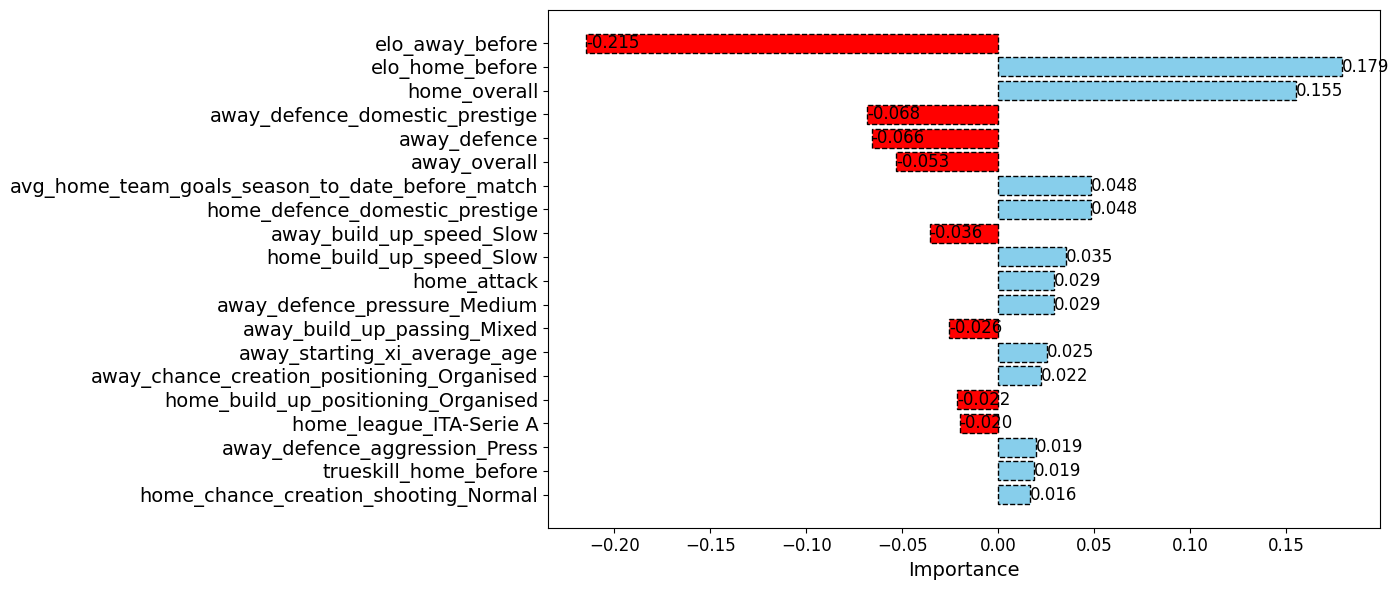
\includegraphics[width=1.12\linewidth]{statics/top20_coeff_importance_lr_selected_features_away.png}
    \caption{Feature Importance for Home Win Prediction}
    \label{fig:feature_importance}
\end{figure}

\subsection{Monte Carlo Simulations}
Simulations were conducted to evaluate bankroll strategies under controlled conditions \ref{fig:monte_carlo} \ref{tab:final_bankroll}.

\begin{figure}[h]
    \centering
    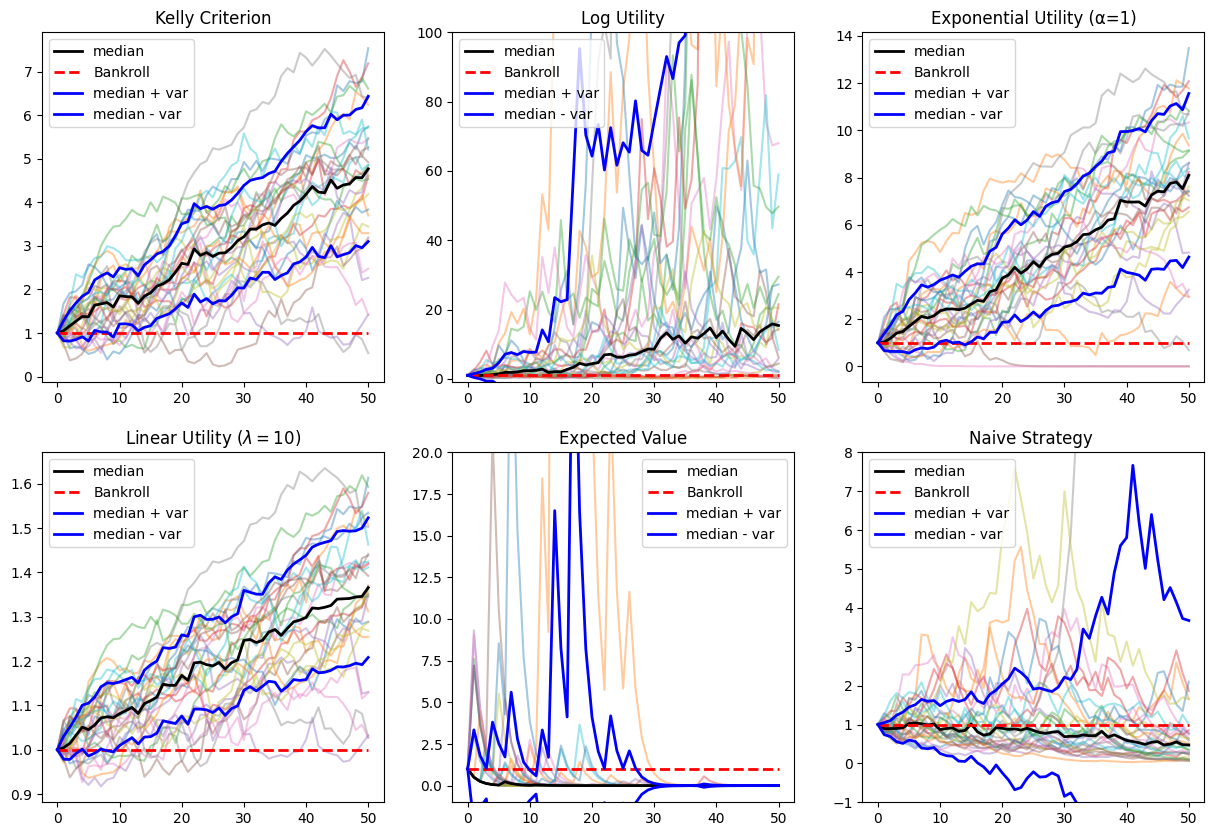
\includegraphics[width=\linewidth]{statics/monte_carlo_b=b.png}
    \caption{Monte Carlo Simulation Results for Different Strategies}
    \label{fig:monte_carlo}
\end{figure}

\begin{table}[h]
\centering
\scalebox{0.8}{%
\begin{tabular}{lccccc}
\toprule
\textbf{Strategy} & \textbf{Mean} & \textbf{Std Dev} & \textbf{Min} & \textbf{Max} & \textbf{Sharpe R.} \\
\midrule
Kelly Criterion & 4.48 & 1.67 & 0.54 & 7.54 & \textbf{0.30} \\
Log Utility & \textbf{270.85} & 983.14 & 0.19 & \textbf{5414.01} & 0.29 \\
Exponential Utility & 7.46 & 3.46 & 0.00 & 13.48 & 0.25 \\
Linear Utility & 1.35 & \textbf{0.16} & \textbf{1.03} & 1.61 & \textbf{0.30} \\
Naive Strategy & 1.20 & 3.20 & 0.06 & 18.19 & 0.01 \\
\bottomrule
\end{tabular}%
}
\caption{Final Bankroll Statistics from Simulations}
\label{tab:final_bankroll}
\end{table}

\subsection{Online Testing}
A real-world testing phase was conducted over five weeks, focusing on matches from top European leagues \ref{fig:capital_evolution} \ref{tab:strategy_performance}.

\begin{figure}[h]
    \centering
    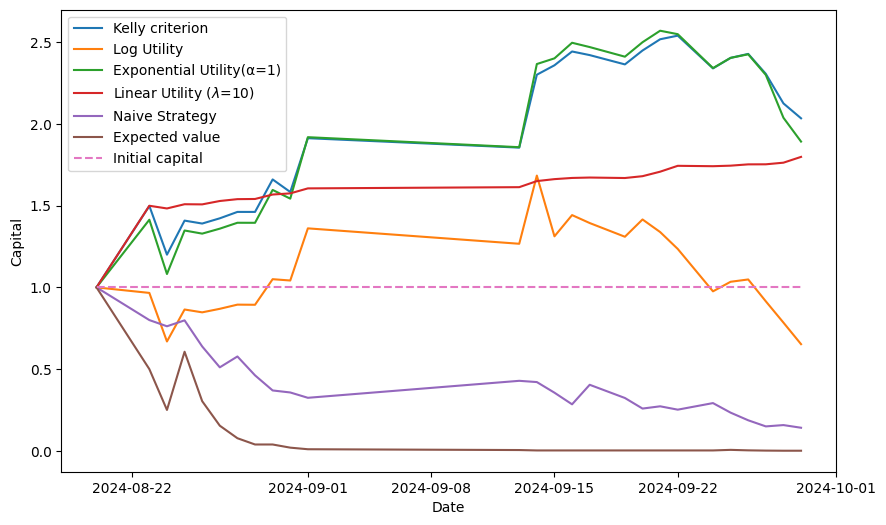
\includegraphics[width=\linewidth]{statics/bankroll_evolution2.png}
    \caption{Capital Evolution During Online Testing}
    \label{fig:capital_evolution}
\end{figure}

\begin{table}[h]
\centering
\scalebox{0.8}{%
\begin{tabular}{lccc}
\toprule
\textbf{Strategy} & \textbf{Final B.} & \textbf{Mean Growth (\%)} & \textbf{Std Dev (\%)} \\
\midrule
Kelly Criterion & \textbf{2.034} & \textbf{2.034} & 8.923 \\
Exponential Utility & 1.892 & 1.886 & 10.309 \\
Linear Utility & 1.798 & 1.776 & \textbf{5.360} \\
Log Utility & 0.653 & -2.129 & 26.516 \\
Naive Strategy & 0.141 & -24.299 & 52.419 \\
\bottomrule
\end{tabular}%
}
\caption{Strategy Performance Metrics}
\label{tab:strategy_performance}
\end{table}

\section{Discussion}
The Kelly Criterion and Exponential Utility strategies consistently outperformed others, nearly doubling the initial bankroll in both simulations and online testing. These strategies effectively balance risk and return by optimizing the utility functions that account for risk preferences.

The Linear Utility strategy provided steady growth with minimal volatility, making it suitable for risk-averse bettors. The Log Utility strategy was overly conservative, failing to capitalize on profitable opportunities.

Simpler strategies like the Naive and Expected Value approaches underperformed, highlighting the importance of sophisticated bankroll management in sports betting.

\subsection{Limitations}

Our static framework simplifies optimization but limits interpretation of long-term gains and variance by ignoring intertemporal dependencies and bankroll evolution. The predictive model could be enhanced with more features, hyperparameter tuning, and complex models like deep learning to capture dynamic patterns. Fixed risk aversion parameters reduce adaptability; dynamic risk preferences could improve strategy responsiveness. The five-week testing period was short and limited in scope, possibly not reflecting long-term performance in diverse markets.

\subsection{Future Work}

Future work involves extending testing periods and scope, enhancing the predictive model with additional data and dynamic modeling for improved accuracy, developing a dynamic optimization framework to better manage long-term gains and variance, and introducing adaptive risk preferences responsive to changes in wealth and market conditions.

\section{System Deployment}
A microservices architecture was adopted, with services containerized using Docker and orchestrated with Kubernetes. The system was deployed on Azure Kubernetes Service (AKS), leveraging cloud infrastructure for scalability and reliability \ref{fig:system_architecture}.

\begin{figure}[!htbp]
    \centering
    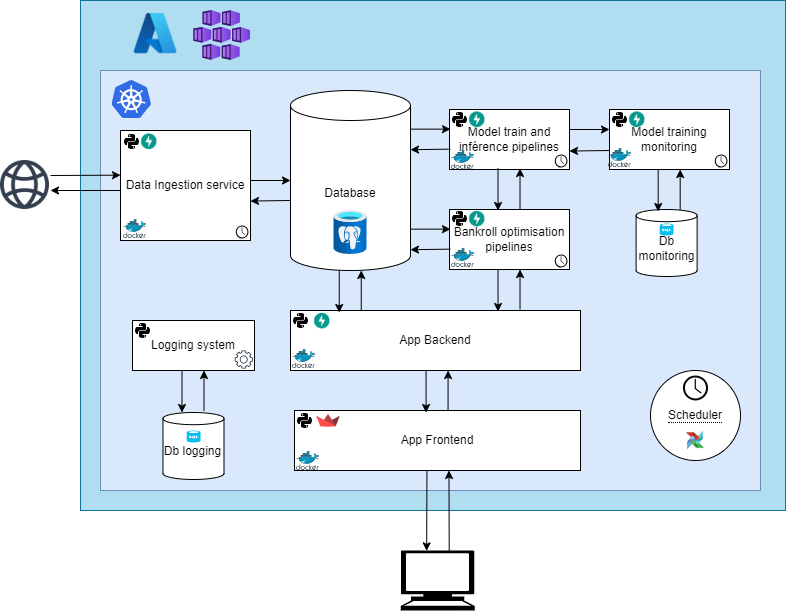
\includegraphics[width=0.9\linewidth]{statics/diagrem_archi_services.png}
    \caption{System Architecture Deployed on AKS}
    \label{fig:system_architecture}
\end{figure}

\section{Conclusion}
Integrating predictive modeling with advanced bankroll management strategies significantly enhances profitability in sports betting. The proposed system demonstrates the practical application of mathematical and computational techniques to real-world betting scenarios, achieving superior performance compared to traditional methods.

\end{document}